% Saimiri museum-microCT (USNM 194346) + VALiDATe29 squirrel-monkey brain
% atlas. Geometry-only pillar (deliverables 1-2): the museum skull and the
% atlas are both staged and the geometry is measured end-to-end; the
% quantitative acoustics stay guarded (no HU-calibrated colony CT). Build:
%   python docs/saimiri/make_figures.py   # regenerate figures from the cache
%   pdflatex manuscript
%   pdflatex manuscript

\documentclass{compactarticle}

\usepackage{amsmath,amssymb,amsfonts,bm}
\usepackage{graphicx}
\usepackage[utf8]{inputenc}
\usepackage[T1]{fontenc}
\usepackage{booktabs}
\usepackage{enumitem}
\usepackage{xcolor}
\usepackage{float}
\usepackage{ragged2e}
\usepackage{url}

\graphicspath{{figures/}}

\providecommand{\br}{\toprule}
\providecommand{\mr}{\midrule}
\providecommand{\TODO}[1]{\textcolor{red!75!black}{\textbf{[TODO]} #1}}

\begin{document}
\justifying
\fancyhead[R]{\small\itshape Squirrel-monkey skull + VALiDATe29 pillar}

\articletype{Design \& setup report}

\title{A transcranial focused-ultrasound targeting pipeline for the
       squirrel monkey: a \emph{Saimiri sciureus} museum microCT
       registered to the VALiDATe29 brain atlas, with a hard
       CT-calibration guard (deliverables 1--2)}

\author{Gianmarco F Pinton}

\affil{Joint Department of Biomedical Engineering, University of North
       Carolina at Chapel Hill and North Carolina State University}

\email{gia@email.unc.edu}

\keywords{transcranial focused ultrasound, squirrel monkey,
          \emph{Saimiri sciureus}, VALiDATe29, HU calibration,
          somatosensory cortex, points per wavelength}

\begin{abstract}
We document the fifth pillar of TUBA --- a transcranial focused
ultrasound (FUS) pipeline for the common squirrel monkey
(\emph{Saimiri sciureus}), prepared for NIH R01 EB037345 (Aim~3):
per-animal skull models for time-reversal aberration correction and
multifocal beam design targeting the hand representations of primary
somatosensory (S1 areas 3b and 1) and primary motor (M1, area 4)
cortex. This report covers \textbf{deliverables 1--2 (the geometry
stages)} and is scoped, by design decision, to a \emph{geometry-only}
build: no HU-calibrated colony CT is available yet, so the pillar is
bootstrapped on an \emph{uncalibrated} museum microCT
(squirrel monkey \emph{Saimiri sp.}, NMNH USNM~194346, MorphoSource
media 000116521, UTCT; 490 slices, 0.0977\,mm in-plane $\times$
0.1189\,mm slice) registered to the VALiDATe29 multi-channel MRI
atlas of the squirrel-monkey brain (Schilling \emph{et al.}\ 2017;
29 animals, histologically-defined cortical labels). \textbf{Both the
skull and the atlas are staged and the geometry is now measured
end-to-end}: the anisotropic microCT is isotropised to 0.0977\,mm, its
orientation is confirmed clean RAS, and an endocranial cavity of
25.35\,mL is extracted whose boundary sits on the inner table
(0.26\,mm mean gap to bone) --- which required diagnosing that this
scan's field of view clips the occiput, breaking an assumption in the
shared cavity extractor. The \texttt{cavity\_binary} SyN to the atlas
brain mask then fits to Dice~0.979, warping the region-level labels
(confirmed \emph{region-level} --- S1 = anterior parietal cortex,
M1 = primary motor cortex, l/r separate) back to subject-space S1/M1
targets that are anatomically correct (M1 rostral and dorsal to S1,
5.2\,mm apart). The pillar reuses
TUBA's core primitives from the mouse/rat/macaque pillars almost
unchanged --- bone-shell cavity extraction
(\texttt{tuba.core.cavity.bone\_shell\_cavity}), \texttt{cavity\_binary}
ANTs SyN (affine\,+\,deformable), atlas-into-subject warp, and the
beam-aligned $(c,\rho)$ slab export. Its \emph{distinctive}
contribution is the \textbf{CT-calibration guard} for
deliverable~1: a new module \texttt{tuba.core.hu\_acoustics} implements
the Aubry (2003) porosity HU$\,\to\,(\rho,c,\alpha)$ model but
\emph{refuses to run} on input not flagged Hounsfield-calibrated
(\texttt{UncalibratedInputError}), so a museum microCT can never
silently produce quantitatively wrong acoustics; an
explicitly-flagged placeholder ramp is the sanctioned geometry-only
fallback. Deliverable~1 also reports the points-per-wavelength (PPW)
budget across the 2--4\,MHz operating band on the simulation grid, and
a grid-convergence run of the transcranial time-of-flight aberration
(the scalar a time-reversal correction must undo), which converges to
0.24\,\% between $60$ and $30\,\mu$m. The scan-dependent constants
(orientation flips, intensity thresholds, cavity hull geometry) are now
\emph{calibrated} against the staged scan, and the cavity, registration,
target, and placement outputs and their QC figures are produced by the
end-to-end driver.
The downstream wave physics (deliverables 3--7: time-reversal,
multifocal synthesis, the two-foci feasibility sweep, MI/bioheat
safety, and the per-animal export artifact) is out of scope for this
branch and consumes the $(c,\rho,dz)$ slab in the \texttt{fullwave2-*}
solver siblings. Code: \texttt{src/tuba/species/saimiri.py},
\texttt{tuba.core.hu\_acoustics}, \texttt{tuba.atlases.validate29};
data manifest + fetchers at \texttt{src/tuba/data/}.
\end{abstract}

% =============================================================================
\section{Scope and status}
\label{sec:scope}

Like the four prior TUBA pillars (mouse, macaque, human, rat), this one
is now calibrated end-to-end against a staged scan --- with a measured
cavity volume, a fitted registration, and subject-space targets --- but
with one deliberate boundary: the acoustics are \emph{geometry-only}.
The funded project targets a Vanderbilt colony whose HU-calibrated CT is
not yet in hand, so we build and verify the full geometry on a public
museum microCT and gate the quantitative acoustics behind a calibration
guard (\S\ref{sec:acoustic}) so nothing downstream mistakes an
uncalibrated skull for a quantitative one. Two decisions frame the
branch:
\begin{enumerate}[leftmargin=*]
\setlength\itemsep{0pt}
  \item \textbf{Subject data:} a public museum microCT
        (\S\ref{sec:source}), geometry only. The HU$\to$acoustics step
        refuses to run on it.
  \item \textbf{Scope:} deliverables 1--2 (CT$\to$acoustic model +
        atlas registration + target export + QC). Deliverables 3--7
        (the wave-solver study) are out of scope here and live in the
        \texttt{fullwave2-*} siblings (\S\ref{sec:scope-out}).
\end{enumerate}
Both the museum skull (\S\ref{sec:source}) and the VALiDATe29 atlas
(\S\ref{sec:atlas}) are staged; all geometry numbers below are measured
from them.

% =============================================================================
\section{Source data}
\label{sec:source}

\paragraph{Skull.} The skull volume is a microCT scan of a squirrel
monkey (\emph{Saimiri sp.}) cranium, museum specimen USNM~194346
(National Museum of Natural History), scanned at the University of Texas
High-Resolution X-ray CT Facility (UTCT, ACTIS scanner) and distributed
as MorphoSource media 000116521~\cite{morphosource-saimiri} (also on
DigiMorph~\cite{digimorph-saimiri}). The reconstruction is 490 axial
slices, $504\times422$\,px, 16-bit, \emph{anisotropic} at 0.0977\,mm
in-plane $\times$ 0.1189\,mm slice --- a dry cranium, no soft tissue.
Part of the openVertebrate / oUTCT collection the TUBA macaque
pillar~\cite{tuba-macaque} also draws from (Copes \emph{et
al.}\ 2016~\cite{copes-2016}). The MorphoSource record's taxonomy is
internally inconsistent (catalogue field \emph{S.~boliviensis};
Rossie's scan description \emph{S.~sciureus sciureus}, male) --- genus
\emph{Saimiri} either way. Table~\ref{tab:scan-params} summarises the
parameters.

\begin{table}[H]
\centering
\caption{Saimiri USNM~194346 (MorphoSource media 000116521) scan
         parameters, from the media manifest. The intensity axis is
         \emph{uncalibrated} (no HU phantom in the field of view).}
\label{tab:scan-params}
\small
\begin{tabular}{ll}
\br
Specimen & \emph{Saimiri sp.}, USNM~194346 (NMNH) \\
MorphoSource media & 000116521 (ark:/87602/m4/M116521) \\
Facility & UT Austin High-Resolution X-ray CT (UTCT ACTIS) \\
Slices & 490 axial, $504\times422$\,px, 16-bit \\
Voxel & 0.0977\,mm in-plane $\times$ 0.1189\,mm slice (anisotropic) \\
Working pitch & 0.0977\,mm isotropic (slice axis up-sampled) \\
Calvarium thickness & 1.0--1.5\,mm ($\sim$10--15 voxels) \\
Intensity & uncalibrated 16-bit reconstruction counts \\
\mr
\end{tabular}
\end{table}

\paragraph{The occiput is cropped.}
One property of this reconstruction matters downstream and is easy to
miss: the field of view \emph{clips the back of the skull}. Bone mass
per slice is still rising at the last slice of the stack (${\sim}13$k
voxels above the bone threshold, the largest of the posterior range)
rather than tapering to zero as it does at the rostral end. The occiput
therefore continues beyond the scanned volume. This is invisible in a
volume-rendering, but it breaks the ``every row of the skull has bone at
both ends'' assumption the shared cavity extractor relies on
(\S\ref{sec:geometry}), and it is the reason the pillar needs the
\texttt{seal\_floor\_gaps} path. It also means the caudal-most
endocranial geometry is bounded by the scan, not by the specimen.

\paragraph{Anisotropy $\to$ isotropic working cache.}
The shared cavity/align/slab tools (calibrated on the isotropic
rat/mouse museum scans) assume isotropic voxels, so
\texttt{downsample\_to\_working} isotropises the staged stack: it
reformats to RAS at the in-plane pitch with the shared TIFF streamer,
then up-samples \emph{only} the coarse slice axis
(0.1189$\to$0.0977\,mm, order-1) to a 0.0977\,mm isotropic cache.
Up-sampling (never down-sampling) that axis cannot erode the thin
cortical-bone shell, and the whole downstream isotropic pipeline is then
exact, with no change to the shared code.

\paragraph{Uncalibrated intensity --- the central caveat.}
Museum microCT carries no hydroxyapatite/HU phantom, so voxel values
are arbitrary reconstruction counts, not Hounsfield units. Every prior
TUBA pillar faces the same issue and handles it by anchoring a
histogram-relative intensity$\to(c,\rho)$ ramp on the cortical-bone
mode~\cite{tuba-mouse,tuba-macaque}: robust to detector scale, but
explicitly \emph{not} quantitatively calibrated. For the squirrel
monkey we make that limitation a hard boundary rather than a footnote
(\S\ref{sec:acoustic}): the scan is flagged
\texttt{UNCALIBRATED\_MICROCT} and quantitative acoustics are refused.

\paragraph{Wavelength / PPW criterion.}
The neuromodulation operating point is $f_0 = 2$\,MHz with a 2--4\,MHz
design range. The most restrictive wavelength is in the water column
at 4\,MHz: $\lambda_{\min} = c_{\text{water}}/f = 1500/4\times10^{6} =
0.375$\,mm. A finite-difference solve wants $\gtrsim 6$ points per
wavelength there, so the simulation grid pitch is set to
$\Delta x = 60\,\mu$m (\texttt{SIM\_DX\_M} in
\texttt{tuba.species.saimiri}); the resulting PPW budget is
Table~\ref{tab:ppw}. Note the 0.0977\,mm microCT working cache is
\emph{coarser} than the $60\,\mu$m sim grid, so the skull is up-sampled
onto the sim grid by the slab sampler (\S\ref{sec:placement}) --- the
geometry is faithful; only the absolute acoustics are placeholder.

\begin{table}[H]
\centering
\caption{Points-per-wavelength budget on the $\Delta x = 60\,\mu$m
         simulation grid, using the shortest (water) wavelength at each
         frequency (\texttt{tuba.core.hu\_acoustics.report\_ppw}). All
         three bands clear the 6-PPW floor.}
\label{tab:ppw}
\small
\begin{tabular}{rrr}
\br
Frequency & $\lambda_{\text{water}}$ (mm) & PPW @ $60\,\mu$m \\
\mr
2.0\,MHz & 0.750 & 12.50 \\
3.0\,MHz & 0.500 & 8.33 \\
4.0\,MHz & 0.375 & 6.25 \\
\mr
\end{tabular}
\end{table}

% =============================================================================
\section{VALiDATe29 reference atlas}
\label{sec:atlas}

The brain anatomy is provided by the VALiDATe29 atlas of the squirrel
monkey brain~\cite{validate29}, built from 29 animals at the Vanderbilt
University Institute of Imaging Science and distributed CC~BY via NITRC
(RRID:SCR\_015542). Unlike the subject skull, \textbf{the atlas is
staged and validated in this report}: \texttt{tuba.data.fetch\_validate29}
discovers the current file-release link from the NITRC project page
(reusing the WHS click-through of the rat pillar~\cite{tuba-rat}) and
unpacks it under \texttt{\$VALIDATE29\_DEST}; the fetch was exercised
end-to-end here (v1.2 release, 30.4\,MB). Every volume is $212^3$ at
0.300\,mm isotropic. VALiDATe29 is multi-channel: in-vivo anatomical
templates ($T_2$, $T_1$, proton-density), diffusion templates (FA, MD),
an ex-vivo structural\,+\,FA template, a \emph{shipped brain mask}
(\texttt{VALiDATe-brainmask}, ${\sim}33$\,mL) and a discrete
cortical\,+\,white-matter label volume (\texttt{VALiDATe3-labels}; 86
label ids) co-registered from Nissl/myelin sections. It supersedes the
earlier single-subject squirrel-monkey MRI atlas~\cite{gao-2014}.
Figure~\ref{fig:atlas} shows the $T_2$ template, brain mask, and
cortical labels through the brain-mask centroid.

\begin{figure}[H]
\centering
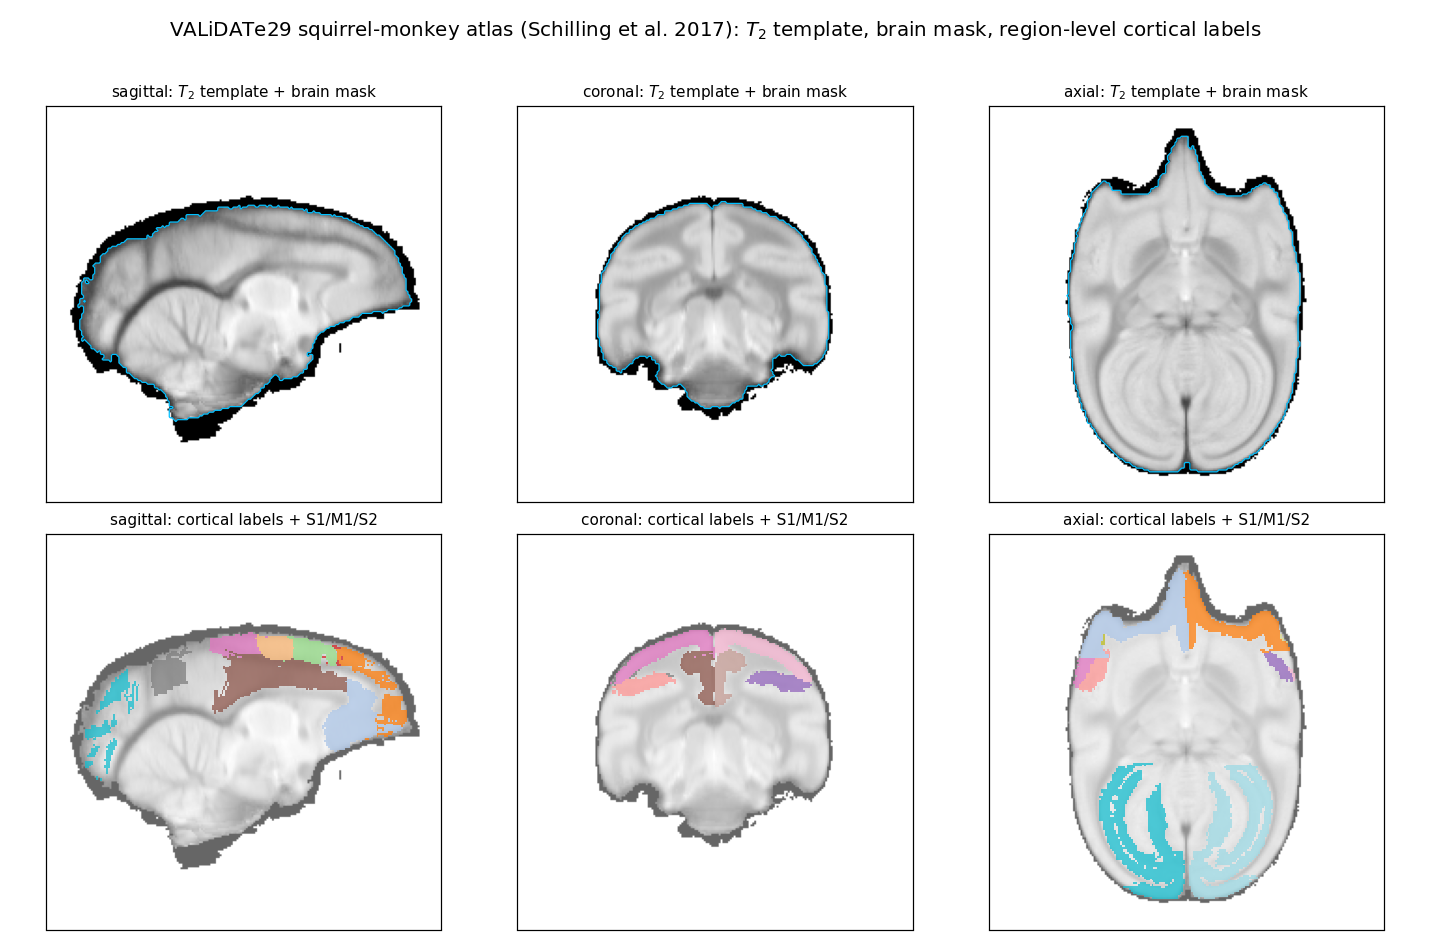
\includegraphics[width=\textwidth]{validate29_atlas.png}
\caption{VALiDATe29 squirrel-monkey atlas through the brain-mask
         centroid (staged v1.2). \textbf{Top}: $T_2$ template with the
         shipped brain-mask contour (blue). \textbf{Bottom}: region-level
         cortical labels (gray-matter ids 1--18) over the template, with
         the S1 (anterior parietal cortex), M1 (primary motor cortex),
         and S2 (PV/S2) target markers where the centroid slice
         intersects them. The squirrel monkey is near-lissencephalic, so
         the cortical areas form broad dorsolateral bands. Generated by
         \texttt{docs/saimiri/make\_figures.py} from the staged atlas.}
\label{fig:atlas}
\end{figure}

\paragraph{Layout tolerance (a real calibration note).}
The staged \texttt{VALiDATe29.zip} double-nests
\texttt{VALiDATe29/VALiDATe29/} and carries macOS
\texttt{\_\_MACOSX}\,/\,\texttt{.\_} resource-fork cruft, and its lookup
table is a plain space-delimited \texttt{id name ABBREV} text file (not
ITK-SNAP format) sitting beside a \texttt{LICENSE.txt}. The binding
\texttt{tuba.atlases.\allowbreak validate29.\allowbreak VALiDATe29}
walks the tree recursively, \emph{ignores the cruft}, resolves the
template/label/mask by keyword, prefers a \texttt{label}-named table
over \texttt{LICENSE}, and raises with the candidate list rather than
guessing --- all confirmed against the staged files. The cavity-binary
registration uses the shipped brain mask directly as its fixed image
(no derive step, no ANTs). Paths are overridable by constructor
argument or environment variable (\texttt{VALIDATE29\_DEST},
\texttt{VALIDATE29\_URL}).

\paragraph{Target structures (confirmed against the staged LUT).}
The study targets the \emph{hand} representations in S1 (areas 3b, 1)
and M1; S1 and M1 are only ${\sim}2$--3\,mm apart in the squirrel
monkey, which is what makes the downstream two-foci feasibility
question (\S\ref{sec:scope-out}) non-trivial. Inspecting the staged
label table settles an important granularity point:
\textbf{VALiDATe29's histological parcellation is region-level, not
Brodmann-area-level.} There is no separate ``area 3b''\,/\,``area
1''\,/\,``area 4'' label; the primary somatosensory hand areas 3a/3b/1/2
are bundled into a single \emph{anterior parietal cortex} (APC) label
and the primary motor cortex is one label, with left and right as
\emph{separate} label ids. The binding maps the study targets
accordingly ($\text{S1}\to$APC, $\text{M1}\to$primary motor,
$\text{S2}\to$PV) and is hemisphere-aware. The atlas-space centroids
measured from the staged label volume (Table~\ref{tab:targets}) are
anatomically consistent: M1 sits rostral and slightly dorsal to S1
across the central sulcus, with clean L/R mirror symmetry. Splitting 3b
from area 1, or isolating the hand knob within APC, needs a stereotaxic
prior on the homunculus that the distributed label volume does not carry
(\S\ref{sec:open}).

\begin{table}[H]
\centering
\caption{VALiDATe29 study-target labels and their \emph{atlas-space}
         centroids (left hemisphere; right is the mirror), measured from
         the staged \texttt{VALiDATe3-labels} volume via
         \texttt{tuba.atlases.validate29}. Coordinates in the atlas RAS
         frame (mm).}
\label{tab:targets}
\small
\begin{tabular}{llrrr}
\br
Target & Atlas label (l/r id) & centroid $(x,y,z)$ & vox & mL \\
\mr
S1 & anterior\_parietal\_cortex (11/12) & $(-10.1,\,1.1,\,10.3)$ & 18\,166 & 0.49 \\
M1 & primary\_motor\_cortex (3/4)       & $(-7.4,\,5.8,\,12.0)$  & 11\,810 & 0.32 \\
S2 & parietal\_ventral\,/\,S2 (7/8)     & $(-13.5,\,3.7,\,4.6)$  & 8\,755  & 0.24 \\
\mr
\end{tabular}
\end{table}

% =============================================================================
\section{Deliverable 1: CT $\to$ acoustic model, with a calibration guard}
\label{sec:acoustic}

This is the pillar's distinctive contribution and the reason a
geometry-only build is safe. The module
\texttt{tuba.core.hu\_acoustics} provides a \emph{quantitative} HU
mapping and a hard guard around it.

\paragraph{Porosity model.}
For Hounsfield-calibrated input we use the Aubry
(2003)~\cite{aubry-2003} porosity model. Bone porosity is estimated
from CT radiodensity,
\begin{equation}
\Phi(\mathrm{HU}) = 1 - \mathrm{clip}\!\left(
   \frac{\mathrm{HU}-\mathrm{HU}_{\text{water}}}
        {\mathrm{HU}_{\text{bone}}-\mathrm{HU}_{\text{water}}},\,0,\,1\right),
\end{equation}
with $\Phi = 1$ water/marrow and $\Phi = 0$ dense cortical bone, and
the acoustic properties interpolate linearly in the bone fraction
$(1-\Phi)$:
\begin{align}
\rho(\Phi) &= \rho_{\text{water}} + (\rho_{\text{bone}}-\rho_{\text{water}})(1-\Phi),\\
c(\Phi)    &= c_{\text{water}} + (c_{\text{bone}}-c_{\text{water}})(1-\Phi),
\end{align}
with cortical endpoints $\rho_{\text{bone}}=1900$\,kg/m$^3$,
$c_{\text{bone}}=2900$\,m/s consistent with the rat/macaque pillars,
and water $\rho=1000$\,kg/m$^3$, $c=1500$\,m/s. Attenuation is taken
proportional to bone fraction between a soft-tissue floor
(0.5\,dB/cm/MHz) and a cortical-bone value
(8\,dB/cm/MHz)~\cite{pinton-2012,pichardo-2011}, reported in
dB/cm/MHz and applied by the downstream solver. SI units throughout.

\paragraph{The guard.}
\texttt{AubryHUMapping.properties()} raises
\texttt{UncalibratedInputError} unless the bound
\texttt{CTCalibration.kind == 'hu'}. The squirrel-monkey scan is a
museum microCT with no phantom, so the pillar binds
\texttt{CT\_CALIBRATION = UNCALIBRATED\_MICROCT} and the quantitative
path is refused by construction. Rather than silently emitting
physically meaningless densities and sound speeds from arbitrary
reconstruction counts, the caller must either (a) supply an
HU-calibrated colony CT --- one line,
\texttt{CT\_CALIBRATION = CTCalibration(kind='hu',
hu\_bone\_max=$\langle$scan$\rangle$)} --- which unlocks the
quantitative mapping automatically, or (b) opt in explicitly to
\texttt{placeholder\_ramp()}, an intensity$\to(c,\rho)$ ramp carrying
nominal cortical endpoints and a \texttt{.placeholder = True} tag so
downstream code can detect the uncalibrated origin. The slab loader
(\S\ref{sec:placement}) uses the flagged placeholder ramp: geometry is
faithful, absolute $(c,\rho)$ are nominal.

\paragraph{PPW report + grid convergence.}
\texttt{acoustic\_model\_report()} prints the calibration state, the
PPW table (Table~\ref{tab:ppw}) at 2/3/4\,MHz on the sim grid, and ---
given a placement and a staged scan --- one grid-convergence run of the
transcranial \emph{time-of-flight aberration}
\begin{equation}
\tau = \int \left(\frac{1}{c(x)} - \frac{1}{c_{\text{ref}}}\right)\,dx,
\end{equation}
the phase-insertion delay that a time-reversal / phase-conjugation
correction must undo, computed along the central beam ray at
$\Delta x$ and $\Delta x/2$ and reported as an absolute and relative
change. On the staged skull, along the beam to the M1 target, this
gives $\tau = -630.2$\,ns at $60\,\mu$m and $-631.7$\,ns at $30\,\mu$m
--- a $1.5$\,ns ($0.24\,\%$) change, i.e.\ the property model is
converged at the sim pitch. This is a convergence of the
acoustic-\emph{property} model
with voxel pitch, not of a full-wave solve (which lives in the solver
siblings, \S\ref{sec:scope-out}); it is exactly the quantity the
downstream aberration correction consumes, so it is the right
model-side convergence to report here. The units and sign are checked
in the offline test suite (homogeneous medium $\Rightarrow \tau = 0$;
a faster bone slab $\Rightarrow \tau < 0$; a smooth profile converges
as $\Delta x \to 0$).

% =============================================================================
\section{Deliverable 2: geometry --- cavity, registration, targets}
\label{sec:geometry}

The geometry stages reuse the rat/macaque dry-skull spine with no
algorithmic change; only the species constants differ, and they are now
calibrated against the staged scan. Figure~\ref{fig:geometry} shows the
result.

\begin{figure}[H]
\centering
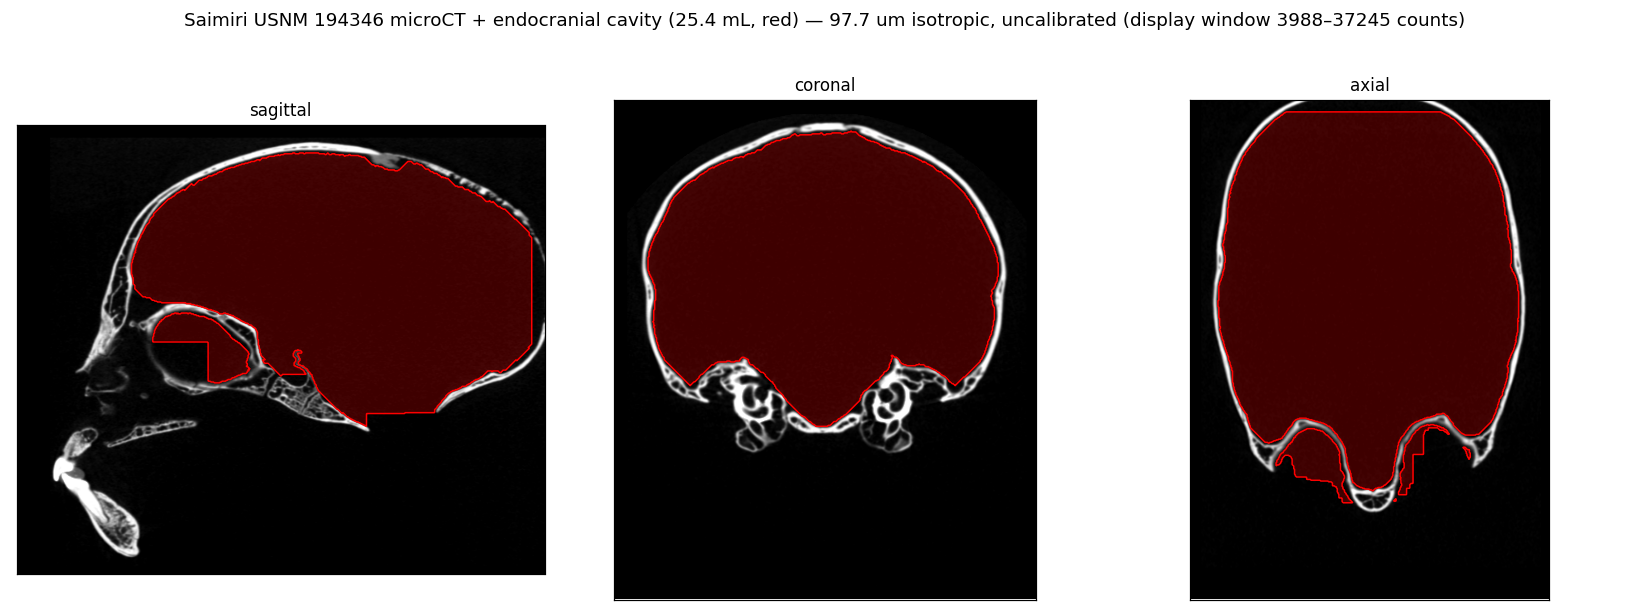
\includegraphics[width=\textwidth]{saimiri_geometry.png}
\caption{Saimiri USNM~194346 microCT (97.7\,$\mu$m isotropic working
         cache) with the extracted endocranial cavity (red contour +
         translucent fill, 25.35\,mL) through the cavity centroid.
         Sagittal, coronal, and axial. The cavity fills the braincase
         from the frontal to the occipital pole and the cerebellar
         fossa, sits on the inner table (0.26\,mm mean gap to bone), is
         bilaterally symmetric, and excludes the orbits --- the shape
         the registration needs. The grey window is taken from the data
         (median to 99.5th percentile, here 3988--37245 counts): a fixed
         ceiling near 16000 would saturate all cortical bone to flat
         white, since air sits at ${\sim}4000$ and cortical bone runs
         past 40000. Uncalibrated intensity (geometry only). Generated
         by \texttt{docs/saimiri/make\_figures.py} from the build
         cache.}
\label{fig:geometry}
\end{figure}

\paragraph{Ingest + orientation (confirmed).}
The MorphoSource TIFF stack carries no DICOM affine; as in the rat
pillar~\cite{tuba-rat} the storage$\to$anatomy mapping is fixed by an
orientation probe (mid-stack orthoslices). The rat/macaque museum-CT
defaults in \texttt{tuba.species.saimiri}
(\texttt{SWAP\_ROW\_COL=True}, \texttt{VOXEL\_SIGNS}$=(-1,-1,+1)$,
storage $(\text{slice}{=}AP,\text{row}{=}DV,\text{col}{=}LR)$) transfer
correctly to this UTCT stack: the probe confirms a clean RAS frame ---
anterior (snout, orbits) at $+y$, dorsal (braincase vault) at $+z$,
bilaterally symmetric about $x$, right-handed --- with no residual tilt
(align angles $0^\circ$, as in rat). True L/R handedness is not
recoverable from a bare museum skull (no fiducial); $+x$ is taken as
Right per RAS and the hemisphere labels carry that caveat.

\paragraph{Endocranial cavity (measured).}
The many dry-cranial openings (orbits, optic canals, foramen magnum)
rule out the mouse-style pure-hysteresis extractor, exactly as in rat
and macaque, so we use the species-agnostic bone-shell extractor
\texttt{tuba.core.cavity.\allowbreak bone\_shell\_cavity} (per-column
basicranium floor + per-row rostral/caudal plugs + per-axial hull), with
a squirrel-scale hull envelope (\texttt{HULL\_X\_HALF\_MM}$=24$, tighter
rostral cutoff at the basicranium than the vault). The cavity shell uses
the same bone threshold as the rest of the pillar
(\texttt{BONE\_LOW}, the histogram air/bone knee), so the cavity
boundary lands on the real inner table.

Two corrections were needed for this scan, and both are worth recording
because they share one root and because the obvious fix is wrong.

The shared recipe builds its shell from surfaces that are only defined
where the bone \emph{brackets} the braincase: a per-row plug needs bone
rostral \emph{and} caudal of the cavity, and a per-column floor needs a
basicranium beneath it. This scan is cropped at the occiput
(\S\ref{sec:source}), and parts of the squirrel-monkey skull base are
thin or absent, so both assumptions fail locally --- and they fail
silently, because the failing row or column still \emph{contains} bone.
\emph{(i)} $22.8\,\%$ of rows never meet posterior bone, so their extent
collapses onto a small rostral structure and the per-row caudal plug
swallows the braincase behind it; the cavity comes out as a hollow shell
whose boundary sits $2.5$\,mm \emph{inside} the inner table.
\emph{(ii)} In columns with no basicranium the first bone encountered
from below is the \emph{vault}, so the floor height jumps to the top of
the head and the floor fills the whole column, punching a
$1.1$\,mL void from skull base to vault through the midline.

Lowering the bone threshold appears to fix (i) --- it thickens the shell
until the leak seals --- but it is a false fix: it insets the cavity
further and yields only $15.9$\,mL. The real fix
(\texttt{seal\_floor\_gaps}) applies one criterion to both surfaces:
a row or column is trusted only if its bone \emph{spans} at least
\texttt{PLUG\_MIN\_SPAN\_MM}$=20$\,mm, and otherwise its bounds are
rebuilt from the nearest row/column that does span. Note that testing
merely whether a row or column \emph{has} bone cannot detect either
failure, for exactly the reason above. The result is insensitive to the
threshold over 20--30\,mm. A per-plane fill
(\texttt{fill\_holes\_2p5d}), which can never claim bone, is retained as
a residual safety net; with the two repairs in place it now contributes
$0.01$\,mL.

The extracted volume is $25.3$\,mL, consistent with a \emph{Saimiri}
whole-brain volume of ${\sim}22$\,mL plus CSF and meninges. Boundary
quality is verified directly rather than by volume alone: the distance
from the cavity boundary to the nearest bone voxel is $0.26$\,mm mean
(median $0.10$, p90 $0.62$), i.e.\ the cavity sits \emph{on} the inner
table, and the centre-fill probe is $1.000$.
Table~\ref{tab:cavity} records the effect of each step; note that the
rejected fix and the two genuine repairs are separated by boundary
quality, not by volume.

\begin{table}[H]
\centering
\caption{Endocranial-cavity extraction on the staged scan. ``Gap'' is
         the distance from the cavity boundary to the nearest bone voxel
         (0 = sitting on the inner table); ``centre fill'' is the cavity
         fraction of a 16\,mm cube at the cavity centroid (1.0 = solid).
         Row 1 is the \emph{rejected} fix: its volume is plausible while
         its boundary is 2.5\,mm off.}
\label{tab:cavity}
\small
\begin{tabular}{lrrr}
\br
Extraction & Volume (mL) & Gap mean/p90 (mm) & Centre fill \\
\mr
Lowered shell threshold (rejected)  & 15.9 & 2.47 / 4.84 & 0.97 \\
Default surfaces (caudal plug swallows) & 16.9 & 1.47 / -- & 0.26 \\
\quad + per-row plug repair          & 24.2 & 0.74 / 1.84 & 0.87 \\
\quad + basicranium floor repair     & 25.34 & --          & -- \\
\quad + per-plane fill (adopted)     & \textbf{25.35} & \textbf{0.26 / 0.62} & \textbf{1.000} \\
\mr
\end{tabular}
\end{table}

\paragraph{Registration --- \texttt{cavity\_binary} SyN
(affine\,+\,deformable).}
Deliverable~2 calls for affine \emph{and} deformable registration, so
--- unlike the macaque/rat pillars, which stop at a 12-DOF Affine --- we
use the full \texttt{cavity\_binary} SyN path
(\texttt{tuba.core.warp.\allowbreak register\_subject\_to\_atlas},
$\mathrm{fixed}=$ VALiDATe29 brain mask, $\mathrm{moving}=$ subject
cavity), the same convention the mouse and mini pillars use. The atlas
template and cortical labels are then pulled back into subject space
through the saved inverse transforms
(\texttt{warp\_atlas\_into\_subject}, linear for the template,
nearest-neighbour for the labels). Unlike the rat and mouse pillars,
which \emph{derive} a brain mask from the annotation, VALiDATe29 ships
its own (\texttt{VALiDATe-brainmask}), so the binding uses it directly
as the SyN fixed image --- no derive step and no ANTs for the mask. On
the staged scan the SyN converges in ${\sim}1$\,min; the fit is
excellent --- the atlas brain mask, warped back into subject space,
overlaps the extracted cavity at \textbf{Dice~0.979}
(25.35 vs 24.9\,mL) and fills the braincase right up to the inner table,
its boundary lying 0.19\,mm from bone on average (p90 0.37\,mm),
Fig.~\ref{fig:qc}. Note the atlas ships a generous intracranial mask
(33.0\,mL, against 14.9\,mL of labelled structures), so the affine
component carries a real scale change to the subject's 25.35\,mL
cavity.

\paragraph{Target export + QC (deliverable 2 outputs).}
\texttt{export\_targets()} writes the S1 (anterior parietal cortex) and
M1 (primary motor cortex) coordinates in the subject simulation frame to
\texttt{saimiri\_targets.json}, alongside the transform prefix (saved
under \texttt{\$TUBA\_SAIMIRI\_REG\_DIR} as
\texttt{saimiri\_cavity\_to\_validate29}), and \texttt{qc\_figure()}
writes the three-panel overlay of Figure~\ref{fig:qc}. The subject-space
left-hemisphere centroids (Table~\ref{tab:subject-targets}) are
anatomically correct: \textbf{M1 sits $4.2$\,mm rostral and $1.6$\,mm
dorsal to S1}, $5.2$\,mm centroid-to-centroid, both in the left
hemisphere --- the sensorimotor topology the study depends on, carried
through the cavity registration from the confirmed atlas-space labels
(Table~\ref{tab:targets}). The centroid separation is larger than the
${\sim}2$--3\,mm quoted for the \emph{hand} representations because
these are whole-region centroids (all of APC vs all of M1), not hand
sub-fields; resolving those needs the stereotaxic prior of
\S\ref{sec:open}.

\begin{table}[H]
\centering
\caption{Study-target centroids in the \emph{subject} aligned-native RAS
         frame (left hemisphere), from \texttt{saimiri\_targets.json}
         --- the atlas labels of Table~\ref{tab:targets} warped through
         the cavity SyN. Volumes scale with the cavity/atlas affine.}
\label{tab:subject-targets}
\small
\begin{tabular}{llrr}
\br
Target & Atlas label (id) & subject centroid $(x,y,z)$ & mL \\
\mr
S1 & anterior\_parietal\_cortex (11) & $(-9.1,\,-5.0,\,16.9)$ & 0.34 \\
M1 & primary\_motor\_cortex (3)      & $(-6.5,\,-0.8,\,18.4)$ & 0.23 \\
\mr
\end{tabular}
\end{table}

\begin{figure}[H]
\centering
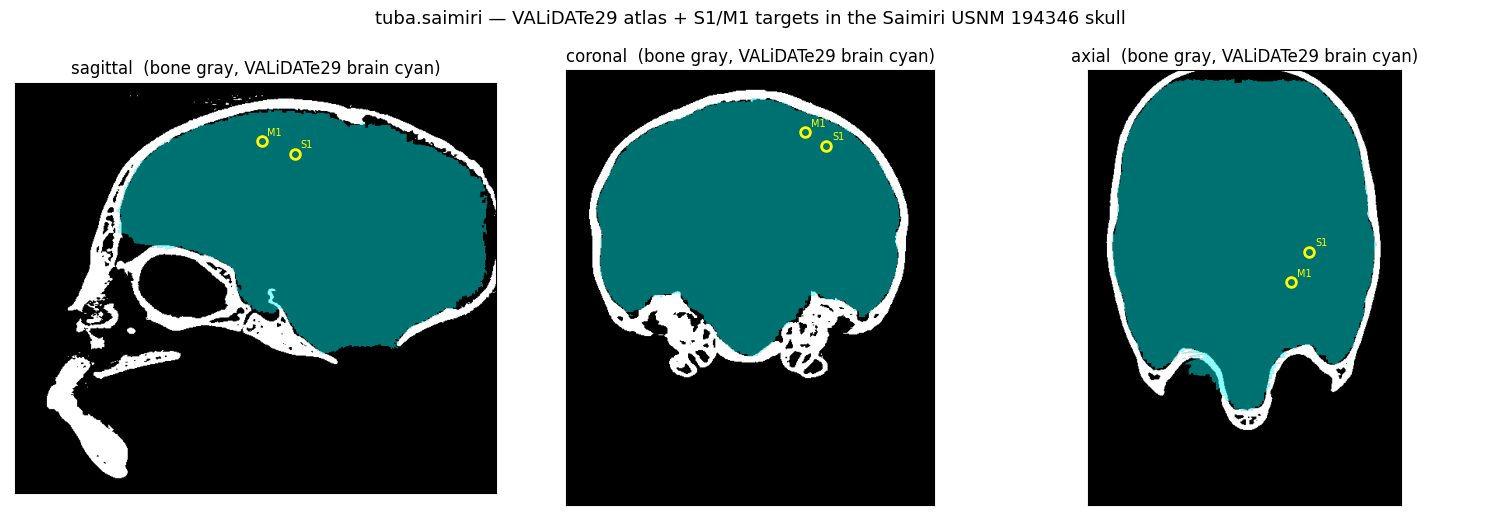
\includegraphics[width=\textwidth]{saimiri_atlas_in_skull.png}
\caption{Deliverable-2 QC: VALiDATe29 atlas registered into the Saimiri
         USNM~194346 skull. Bone shell (gray), the warped VALiDATe29
         brain mask (cyan) filling the braincase, and the S1/M1 target
         markers, in sagittal, coronal, and axial. The warped brain
         fills the braincase to the inner table (0.19\,mm mean gap to
         bone), and M1 lies rostral and dorsal to S1 in the left
         hemisphere across all three planes.
         Cavity vs warped-brain Dice $=0.979$. Generated by
         \texttt{docs/saimiri/make\_figures.py} /
         \texttt{tuba.species.saimiri.qc\_figure}.}
\label{fig:qc}
\end{figure}

% =============================================================================
\section{Placement and slab export}
\label{sec:placement}

\texttt{place\_on\_skull} computes the apex/target/beam triple for a
focused bowl aimed at a study target, and \texttt{load\_slab} returns
$(c,\rho,dz_{\text{slab}},\text{frame})$ with the \emph{same signature}
as the mouse/rat/macaque loaders, so any FDTD or angular-spectrum
driver wired against one species runs on this one unchanged. On the
staged skull, aiming at the M1 target, it lands the bowl apex on the
outer-bone surface, lifts it $11.2$\,mm for scalp clearance, and returns
a $20$\,mm apex-to-target standoff with the beam axis
$\hat{\bm n}=(-0.12,\,0.09,\,-0.99)$ (near-vertical, entering the dorsal
vault). The slab ramp is the flagged placeholder (\S\ref{sec:acoustic});
the cavity is overwritten with brain-parenchymal properties
($c=1540$\,m/s, $\rho=1040$\,kg/m$^3$) exactly as in the other pillars.
This slab is the hand-off boundary to the wave-solver siblings.

% =============================================================================
\section{Out of scope here: the wave-physics study (deliverables 3--7)}
\label{sec:scope-out}

TUBA is the geometry/atlas/targeting layer; the wave physics lives in
the \texttt{fullwave2-*} FDTD siblings and consumes the
$(c,\rho,dz)$ slab and placement this pillar exports. The funded
study's remaining deliverables are therefore deliberately \emph{not}
in this branch:
\begin{enumerate}[leftmargin=*]
\setlength\itemsep{0pt}
  \item[D3] time-reversal aberration correction through the individual
        skull (virtual source at each target $\to$ recorded element
        signals $\to$ phase-conjugate transmit delays);
  \item[D4] multifocal beam synthesis --- two simultaneous foci (S1 +
        M1) with independent amplitude control, plus at least one
        alternative to superposed time reversal
        (e.g.\ Gerchberg--Saxton);
  \item[D5] the feasibility study (highest-priority result): sweep
        two-foci separation 1.5--4.0\,mm at 2, 3, 4\,MHz through the
        skull model, reporting $-6$\,dB focal dimensions,
        peak-to-valley contrast, off-target ratio, and transcranial
        focal gain;
  \item[D6] safety margins --- MI at target and skull, and a bioheat
        estimate over the 400\,kPa / 300\,ms / 3\,s duty cycle;
  \item[D7] the per-animal targeting artifact (element delays,
        apodisations, target metadata, safety numbers).
\end{enumerate}
The PPW budget (Table~\ref{tab:ppw}) and the time-of-flight
grid-convergence (\S\ref{sec:acoustic}) are the model-side inputs D3
and D5 will build on.

% =============================================================================
\section{Verification}
\label{sec:tests}

Verification is at two levels: (i) the end-to-end build now runs on the
staged skull + atlas (\texttt{python -m tuba.species.saimiri build}),
producing the cavity, registration (Dice~0.979), subject-space targets,
QC figure, placement, and D1 report of this document; and (ii) offline
unit tests (\texttt{tests/test\_saimiri.py}, 11 tests, no network /
no antspyx / no data) that pin the logic which must hold regardless of a
scan:
\begin{itemize}[leftmargin=*]
\setlength\itemsep{0pt}
  \item importing the pillar stays ANTs-free (ANTs is lazy inside
        \texttt{tuba.core.warp} and the atlas binding);
  \item the calibration guard refuses uncalibrated input on every
        entry point, and the calibrated Aubry mapping is physically
        monotonic (porosity $\downarrow$, $\rho/c/\alpha \uparrow$ with
        HU) with the correct water / cortical endpoints and clamping;
  \item the placeholder ramp is flagged and maps to nominal endpoints;
  \item the PPW, time-of-flight-aberration, and grid-convergence maths
        (homogeneous $\Rightarrow 0$; bone slab $\Rightarrow$ analytic;
        smooth profile converges);
  \item VALiDATe29 file/label resolution and S1/M1 target keyword
        mapping on a synthetic atlas, plus a synthetic affine
        registration round-trip;
  \item the data manifest carries the three Saimiri entries with the
        expected calibration/license semantics.
\end{itemize}
The full repository suite is 41 passing + 1 skipped; \texttt{ruff} is
clean.

\paragraph{Boundary quality, not just volume.}
A cavity volume that falls inside a plausible bracket is \emph{not}
evidence that the segmentation is right: the rejected extraction of
Table~\ref{tab:cavity} produced 15.9\,mL, comfortably inside the range
quoted for \emph{Saimiri} cranial capacity, while its boundary sat
2.5\,mm inside the inner table and it was missing ${\sim}9$\,mL of
braincase. What caught this was a direct geometric check --- the
distance from each cavity-boundary voxel to the nearest bone voxel,
which must be ${\sim}0$ for a shell-bounded cavity --- together with a
centre-fill probe and orthoslice QC read against a data-derived grey
window rather than a fixed one. Both checks are reported by the build
and are the criteria used in Table~\ref{tab:cavity}.

\paragraph{Shared-code safety.}
\texttt{seal\_floor\_gaps} and \texttt{fill\_holes\_2p5d} touch
\texttt{tuba.core.cavity}, which the mouse, rat, macaque and human
pillars all depend on. The flag defaults to \emph{off}, and the
equivalence was checked by execution rather than by inspection: with
\texttt{seal\_floor\_gaps=False} the new
\texttt{bone\_shell\_cavity} is bitwise identical to the previous
implementation --- same mask, same \texttt{info} dict, same verbose
output --- over 233 paired runs spanning synthetic skull geometries,
degenerate inputs (no bone, all bone), the full parameter cross-product
(hull, geodesic propagation, plug smoothing, caudal seal), and the two
real staged microCT volumes (rat, 0 differing voxels of $25.7$M;
Saimiri, 0 of $146.0$M). Re-running each pillar end-to-end reproduces
its published cavity voxel-for-voxel (rat bone-shell seed $1.50$\,mL,
mouse $450$\,mm$^3$, macaque $92.8$\,mL, all with 0 differing voxels).
Only \texttt{tuba.species.saimiri} opts in.

\paragraph{Adversarial review of the new code.}
The repair paths were then reviewed specifically for defects, which
found four worth fixing and is the reason the mechanism above is
described as it is. Most importantly, the \emph{first} version of this
work misattributed the midline void to the caudal plug and gated the
floor repair on whether a column \emph{has} bone --- a predicate that
can never fire, since the offending columns contain the vault. That is
what motivated the span-based criterion used for both surfaces. The
other three were a fallback path that dropped its sentinel assignments
and so unsealed the shell when no row qualified (reachable by a
parameter sweep past 55\,mm), a gate that could emit plugs into rows
containing no bone at all, and a progress line that reported rebuilds
that had not happened and overstated the real count threefold. All four
are fixed and covered by the checks above.

% =============================================================================
\section{Open items}
\label{sec:open}

The geometry is now staged and validated end-to-end (skull:
\S\ref{sec:geometry}, Figs.~\ref{fig:geometry}--\ref{fig:qc}; atlas:
\S\ref{sec:atlas}, Fig.~\ref{fig:atlas}). The remaining items are the
acoustic calibration and the downstream study:
\begin{enumerate}[leftmargin=*]
\setlength\itemsep{0pt}
  \item \textbf{Quantitative acoustics.} When a Vanderbilt colony CT is
        available, set \texttt{CT\_CALIBRATION} to an \texttt{hu}
        calibration to unlock the quantitative Aubry mapping (one line),
        and re-run the grid-convergence with the real property field.
        Until then the acoustics stay guarded and the slab ramp is the
        flagged placeholder.
  \item \textbf{Hand sub-representation.} Add a stereotaxic
        hand-knob prior within anterior parietal cortex (the label
        granularity limit of \S\ref{sec:atlas}) to resolve areas 3b/1
        from the bundled APC label; the region$\to$label mapping itself
        is confirmed and pinned.
  \item \textbf{L/R handedness.} A museum skull carries no L/R fiducial;
        confirm the hemisphere convention against a colony CT with known
        laterality before per-animal targeting.
  \item \textbf{Downstream study.} Hand the exported slab + targets to
        the \texttt{fullwave2-*} siblings for deliverables 3--7
        (\S\ref{sec:scope-out}).
\end{enumerate}

% =============================================================================
\begin{thebibliography}{99}

\bibitem{morphosource-saimiri} J.~Rossie (data), NMNH Division of
  Mammals (specimen),
  ``Skull [CTImageSeries] --- \emph{Saimiri}, USNM~194346,''
  MorphoSource media 000116521, ark:/87602/m4/M116521, UT Austin
  High-Resolution X-ray CT Facility (staged 2026-08-20).
  \url{https://www.morphosource.org/concern/media/000116521}.

\bibitem{digimorph-saimiri} J.~Rossie,
  ``\emph{Saimiri sciureus} (On-line), USNM~194346,''
  Digital Morphology Library (DigiMorph), University of Texas
  High-Resolution X-ray CT Facility.
  \url{https://digimorph.org/specimens/Saimiri_sciureus/194346/}
  (accessed 2026-08-20).

\bibitem{copes-2016} L.~E.~Copes, L.~A.~B.~Lucas, J.~O.~Thostenson,
  H.~E.~Hoekstra, and D.~M.~Boyer,
  ``A collection of non-human primate computed tomography scans housed
  in MorphoSource, a repository for 3D data,''
  \emph{Scientific Data} {\bf 3}, 160001 (2016).
  \url{https://doi.org/10.1038/sdata.2016.1}.

\bibitem{validate29} K.~G.~Schilling, Y.~Gao, I.~Stepniewska,
  T.-L.~Wu, F.~Wang, B.~A.~Landman, J.~C.~Gore, L.~M.~Chen, and
  A.~W.~Anderson,
  ``The VALiDATe29 MRI Based Multi-Channel Atlas of the Squirrel
  Monkey Brain,''
  \emph{Neuroinformatics} {\bf 15}(4), 343--364 (2017).
  \url{https://doi.org/10.1007/s12021-017-9334-0}. RRID:SCR\_015542.

\bibitem{gao-2014} Y.~Gao, A.~Parvathaneni, S.~Schilling,
  \emph{et al.},
  ``A brain MRI atlas of the common squirrel monkey,
  \emph{Saimiri sciureus},''
  \emph{Proc.\ SPIE Medical Imaging} {\bf 9038}, 90380C (2014).
  \url{https://doi.org/10.1117/12.2043669}.

\bibitem{aubry-2003} J.-F.~Aubry, M.~Tanter, M.~Pernot,
  J.-L.~Thomas, and M.~Fink,
  ``Experimental demonstration of noninvasive transskull adaptive
  focusing based on prior computed tomography scans,''
  \emph{J.\ Acoust.\ Soc.\ Am.} {\bf 113}(1), 84--93 (2003).
  \url{https://doi.org/10.1121/1.1529663}.

\bibitem{pinton-2012} G.~Pinton, J.-F.~Aubry, E.~Bossy, M.~Muller,
  M.~Pernot, and M.~Tanter,
  ``Attenuation, scattering, and absorption of ultrasound in the skull
  bone,''
  \emph{Medical Physics} {\bf 39}(1), 299--307 (2012).
  \url{https://doi.org/10.1118/1.3668316}.

\bibitem{pichardo-2011} S.~Pichardo, V.~W.~Sin, and K.~Hynynen,
  ``Multi-frequency characterization of the speed of sound and
  attenuation coefficient for longitudinal transmission of freshly
  excised human skulls,''
  \emph{Phys.\ Med.\ Biol.} {\bf 56}(1), 219--250 (2011).
  \url{https://doi.org/10.1088/0031-9155/56/1/014}.

\bibitem{tuba-mouse} G.~F.~Pinton,
  ``Migrating the 15\,MHz transcranial mouse pipeline from
  DigiMouse to the Maga (UW) 4K microCT,''
  TUBA validation report, \texttt{docs/mouse/manuscript.pdf}.

\bibitem{tuba-macaque} G.~F.~Pinton,
  ``A 500\,kHz transcranial focused-ultrasound pipeline for the
  rhesus macaque dorsal anterior cingulate cortex,''
  TUBA validation report, \texttt{docs/macaque/manuscript.pdf}.

\bibitem{tuba-rat} G.~F.~Pinton,
  ``A transcranial focused-ultrasound pipeline for the rat:
  DigiMorph dry-skull microCT registered to the Waxholm Space
  SD brain atlas v4.01,''
  TUBA validation report, \texttt{docs/rat/manuscript.pdf}.

\end{thebibliography}

\end{document}
